\documentclass[10pt]{beamer}

\usepackage{amsmath,amssymb}
\usepackage{zxjatype}
\usepackage[ipa]{zxjafont}
\usetheme{metropolis}
\usepackage{tikz}
\usepackage{tikzsymbols}
\usepackage{appendixnumberbeamer}
\usepackage{bm}

\usefonttheme{professionalfonts}
\usetikzlibrary{positioning}

% -- block color ---
\setbeamercolor{block title}{use=structure, fg=white!90!purple, bg=purple!75!black}
\setbeamercolor{block body}{use=structure, fg=black!90!white, bg=white!90!black}
\setbeamercolor{block title example}{use=structure, fg=white!90!cyan, bg=cyan!75!black}
\setbeamercolor{block body example}{use=structure, fg=black!90!white, bg=white!90!black}

% --- page number ---
\setbeamertemplate{footline}{%
	\raisebox{10pt}{\makebox[\paperwidth]{\hfill\makebox[7em]{\normalsize\texttt{\insertframenumber/\inserttotalframenumber}}}}%
}

% --- title logo ---

\newcommand{\myinsertlogo}[1]{%
\begin{tikzpicture}[overlay, remember picture]
    \node[above left=1cm and .8cm of current page.south east] {\includegraphics[width=2.25cm]{#1}};
\end{tikzpicture}}

% --- commands ---

\newcommand{\redtext}[1]{\textcolor{red}{#1}}
\newcommand{\bluetext}[1]{\textcolor{blue}{#1}}
\newcommand<>{\greentext}[1]{\alt#2{\textcolor{green}{#1}}{#1}}
\newcommand<>{\highlight}[2][yellow]{%
    \alt#3{%
        \tikz[baseline=(x.base)]{
            \node[rectangle,rounded corners,fill=#1!10](x){$#2$};
        }%
    }{%
        #2
    }%
}

\newcommand<>{\highlightcap}[3][yellow]{%
    \alt#4{%
        \tikz[baseline=(x.base)]{
            \node[rectangle,rounded corners,fill=#1!10](x){$#2$};
            \node[anchor=north, color=#1, align=center] at (x.south) {#3};
        }%
    }{%
        #2
    }%
}

\newcommand<>{\highlightcaphead}[3][yellow]{%
    \alt#4{%
        \tikz[baseline=(x.base)]{
            \node[rectangle,rounded corners,fill=#1!10](x){$#2$};
            \node[anchor=south, color=#1, align=center] at (x.north) {#3};
        }%
    }{%
        #2
    }%
}

\newcommand<>{\highlightcapright}[3][yellow]{%
    \alt#4{%
        \tikz[baseline=(x.base)]{
            \node[rectangle,rounded corners,fill=#1!10](x){$#2$};
            \node[anchor=west, color=#1, align=center] at (x.east) {#3};
        }%
    }{%
        #2
    }%
}

\newenvironment{supframe}[1]{%
    \setbeamercolor{frametitle}{fg=white!90!purple, bg=mLightGreen!75!black}%
    \begin{frame}{#1}%
}{%
    \end{frame}%
}

\newcommand{\nbracket}[1]{\left( #1 \right)}
\newcommand{\cbracket}[1]{\left\{ #1 \right\}}
\newcommand{\rbracket}[1]{\left[ #1 \right]}
\newcommand{\abracket}[1]{\left\langle #1 \right\rangle}

\DeclareMathOperator{\tr}{tr}

\title{Probability Distributions (PRML \S2.3.1-2.3.7)}
\date{PRML Reading Club (June 3, 2019)}
\author{Satoshi Murashige}
\institute{Mathematical Informatics Lab., NAIST}

\begin{document}
    \begin{frame}[plain]
        \maketitle
        \myinsertlogo{naist.pdf}
    \end{frame}
    
    \begin{frame}{Table of Contents}
        \begin{itemize}
            \item Important properties of Gaussian distributions
                \begin{itemize}
                    \item \S2.3.1 Conditional Gaussian Distribution
                    \item \S2.3.2 Marginal Gaussian Distribution
                    \item \S2.3.3 Bayes' theorem for Gaussian variables
                \end{itemize}
            \item Parameter estimation for the Gaussian
                \begin{itemize}
                    \item \S2.3.4 Maximum likelihood for the Gaussian
                    \item \S2.3.5 Sequential estimation
                    \item \S2.3.6 Bayesian inference for the Gaussian
                \end{itemize}
            \item Student's t-distribution
                \begin{itemize}
                    \item \S2.3.7 Students's t-distribution
                \end{itemize}
        \end{itemize}
    \end{frame}
    
    \section{\S2.3.1 Conditional Gaussian Distribution}
    
    \begin{frame}{Completing the square (for univariate case)}
        \begin{itemize}
            \item Basic idea:
                \begin{align*}
                    &x^2 - 6x + 2 \\
                    \onslide<2->{&= \highlight<3->[red]{x^2 - 6x + 9} - 7 \\}
                    \onslide<4->{&= \highlight[red]{(x - 3)^2} - 7}
                \end{align*}
            \item Example:
                \begin{align*}
                    &\exp\left(-\frac{1}{2}x^2 + 2x + \mathrm{const.}\right) \\
                    \onslide<5->{&= \exp\left\{-\frac{1}{2}(x^2 - 4x + 4) + \mathrm{const.}\right\} \\}
                    \onslide<6->{&= \highlightcap<7->[red]{\exp\left\{-\dfrac{(x - 2)^2}{2}\right\}}{\small Unnormalized Gaussian}\cdot\exp(\mathrm{const.}) }
                \end{align*}
        \end{itemize}
    \end{frame}
    
    \begin{frame}{Important properties of Gaussian Distribution}
        Now, we consider to derive the following properties:
        \begin{align*}
            &p(\mathbf x_a, \mathbf x_b) = p(\mathbf x) = \mathcal N(\mathbf x | \bm \mu, \bm \Sigma) 
            \Rightarrow 
            \begin{array}{l}
                 p(\mathbf x_a | \mathbf x_b) = \mathcal N(\mathbf x_a | \bm \mu_{a|b}, \bm \Sigma_{a|b})  \\
                 p(\mathbf x_a) = \mathcal N(\mathbf x_a | \bm \mu_a, \bm \Sigma_a) 
            \end{array}
        \end{align*}
        \begin{center}
            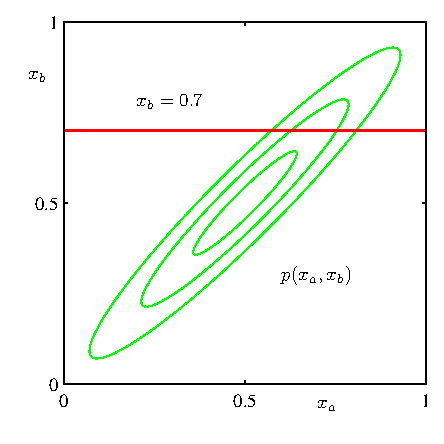
\includegraphics[width=0.45\hsize]{figs/Figure2_9a.pdf}
            \hfill
            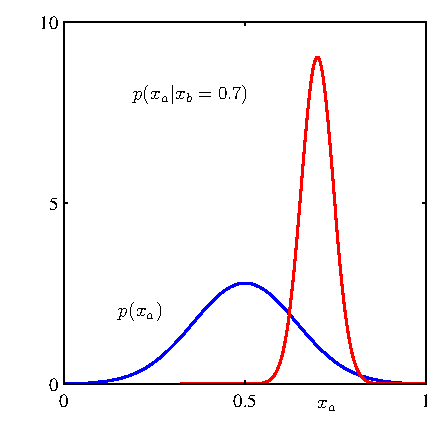
\includegraphics[width=0.45\hsize]{figs/Figure2_9b.pdf} \\
            Figure 2.9
        \end{center}
    \end{frame}
    
    \begin{frame}{Definition of Notation (1/2)}
        Consider a joint distribution $p(\mathbf x) = \mathcal N(\mathbf x | \bm \mu, \bm \Sigma)$
        \begin{itemize}
            \item Separate a $D$-dimensional vector $\mathbf x \sim \mathcal N(\mathbf x | \bm \mu, \bm \Sigma)$
                into $\mathbf x_a \in \mathbb R^M$ and $\mathbf x_b \in \mathbb R^{D-M}$
                \begin{align*}
                    \mathbf x &= \begin{pmatrix}
                        \mathbf x_a \\
                        \mathbf x_b 
                    \end{pmatrix} \tag{2.65}\\
                    \bm \mu &= \begin{pmatrix}
                        \bm \mu_a \\
                        \bm \mu_b 
                    \end{pmatrix} \tag{2.66}\\
                    \bm \Sigma &= \begin{pmatrix}
                        \bm \Sigma_{aa} & \bm \Sigma_{ab} \\
                        \bm \Sigma_{ba} & \bm \Sigma_{bb} 
                    \end{pmatrix} \tag{2.67}
                \end{align*}
            \item The symmetry $\bm\Sigma^\top = \bm\Sigma$ of the covariance matrix, 
                \begin{align*}
                    \bm\Sigma_{aa}^\top = \bm\Sigma_{aa}&, \bm\Sigma_{bb}^\top = \bm\Sigma_{bb} \;\; (\mbox{i.e. symmetry})\\
                    \bm\Sigma_{ba}^\top &= \bm\Sigma_{ab}
                \end{align*}
        \end{itemize}
    \end{frame}

    \begin{frame}{Definition of Notation (2/2)}
        \begin{itemize}
            \item The \textit{precision matrix} $\bm\Lambda$ is convenient in many situations
                \begin{align*}
                    \bm\Lambda &\equiv \bm\Sigma^{-1} \tag{2.68} \\
                    \bm\Lambda &= \begin{pmatrix}
                        \bm \Lambda_{aa} & \bm \Lambda_{ab} \\
                        \bm \Lambda_{ba} & \bm \Lambda_{bb} 
                    \end{pmatrix} \tag{2.69}
                \end{align*}
            \item Because the inverse of a symmetric matrix is also symmetric (proof: ex. 2.22), 
                \begin{align*}
                    \bm\Lambda_{aa}^\top = \bm\Lambda_{aa}&, \bm\Lambda_{bb}^\top = \bm\Lambda_{bb} \;\; (\mbox{i.e. symmetry})\\
                    \bm\Lambda_{ba}^\top &= \bm\Lambda_{ab}
                \end{align*}
            \item NOTE: Generally, for instance, $\bm\Lambda_{aa} \not = \bm\Sigma_{aa}^{-1}$
        \end{itemize}
    \end{frame}
    
    \begin{supframe}{Solution of Exercise 2.22}
        Let $\mathbf A$ be a symmetric matrix ($\mathbf A = \mathbf A^\top$).
        The inverse matrix $\mathbf A^{-1}$ satisfies
        \[
            \mathbf A\mathbf A^{-1} = \mathbf I.
        \]
        By taking the transpose of both sides of this equation, 
        we obtain
        \[
            (\mathbf A^{-1})^\top \mathbf A^\top = \mathbf I.
        \]
        From the definition of inverse matrix, we obtain
        \[
            (\mathbf A^{-1})^\top = \mathbf A^{-1}.
        \]
        Therefore, $\mathbf A^{-1}$ is also symmetric matrix.
    \end{supframe}
    
    \begin{frame}{Derivation of Conditional Gaussian Distribution}
        \begin{block}{Conditional Gaussian Distribution}
            \[
                p(\mathbf x_a, \mathbf x_b) = \mathcal N(\mathbf x | \bm\mu, \bm\Sigma)
                \Rightarrow p(\mathbf x_a | \mathbf x_b) = \mathcal N(\mathbf x_a | \bm\mu_{a|b}, \bm\Sigma_{a|b})
            \]
        \end{block}
        From the product rule of probability, 
        \begin{align*}
            \highlightcap<2->[blue]{p(\mathbf x_a | \mathbf x_b)}{Unknown}
            = \frac{\highlightcaphead<2->[red]{p(\mathbf x_a, \mathbf x_b)}{Known}}{\highlightcap<2->[blue]{p(\mathbf x_b)}{Unknown}}
        \end{align*}
        Take the logarithm of both sides, 
        \begin{align*}
            \ln p(\mathbf x_a | \mathbf x_b) 
            &= \ln p(\mathbf x_a, \mathbf x_b) + \mathrm{const.} \\
            &= -\frac{1}{2}(\mathbf x - \bm\mu)^\top\bm\Sigma^{-1}(\mathbf x - \bm\mu) + \mathrm{const.}
        \end{align*}

    \end{frame}
    
    \begin{frame}{Derivation of Conditional Gaussian Distribution}
        Because (2.70) is a quadratic form of $\mathbf x_a$,
        the corresponding conditional distribution $p(\mathbf x_a | \mathbf x_b)$ will be Gaussian.
        \begin{align*}
            &-\frac{1}{2}(\mathbf x - \bm\mu)^\top \bm\Sigma^{-1}(\mathbf x - \bm\mu) \\
            &=-\frac{1}{2}(\mathbf x_a - \bm\mu_a)^\top \bm\Lambda_{aa}(\mathbf x_a - \bm\mu_a)
            -\frac{1}{2}(\mathbf x_a - \bm\mu_a)^\top \bm\Lambda_{ab}(\mathbf x_b - \bm\mu_b) \\
            &\qquad -\frac{1}{2}(\mathbf x_b - \bm\mu_b)^\top \bm\Lambda_{ba}(\mathbf x_a - \bm\mu_a)
            -\frac{1}{2}(\mathbf x_b - \bm\mu_b)^\top \bm\Lambda_{bb}(\mathbf x_b - \bm\mu_b) \tag{2.70} \\
            %---------------
            \onslide<2->{
            &= -\frac{1}{2}\left( \highlight[red]{\mathbf x_a^\top\bm\Lambda_{aa}\mathbf x_a} - \highlight[red]{\mathbf x_a^\top\bm\Lambda_{aa}\bm\mu_a} - 
                               \highlight[red]{\bm\mu_a^\top\bm\Lambda_{aa}\mathbf x_a} + \bm\mu_a^\top\bm\Lambda_{aa}\bm\mu_a \right) \\
            &\qquad -\frac{1}{2}\left( \mathbf x_a^\top\bm\Lambda_{ab}\mathbf x_b - \highlight[red]{\mathbf x_a^\top\bm\Lambda_{ab}\bm\mu_b} - 
                               \bm\mu_a^\top\bm\Lambda_{ab}\mathbf x_b + \bm\mu_a^\top\bm\Lambda_{ab}\bm\mu_b \right) \\
            &\qquad -\frac{1}{2}\left( \mathbf x_b^\top\bm\Lambda_{ba}\mathbf x_a - \mathbf x_b^\top\bm\Lambda_{ba}\bm\mu_a - 
                               \highlight[red]{\bm\mu_b^\top\bm\Lambda_{ba}\mathbf x_a} + \bm\mu_b^\top\bm\Lambda_{ba}\bm\mu_a \right) \\
            &\qquad -\frac{1}{2}\left( \mathbf x_b^\top\bm\Lambda_{bb}\mathbf x_b - \mathbf x_b^\top\bm\Lambda_{bb}\bm\mu_b - 
                               \bm\mu_b^\top\bm\Lambda_{bb}\mathbf x_b + \bm\mu_b^\top\bm\Lambda_{bb}\bm\mu_b \right) \\
            &= \highlightcap[red]{\displaystyle -\frac{1}{2}\mathbf x_a^\top\bm\Lambda_{aa}\mathbf x_a}{\small The second order term}
                + \highlightcap[red]{\mathbf x_a^\top(\bm\Lambda_{aa}\bm\mu_a + \bm\Lambda_{ab}\bm\mu_b)}{The linear term}
                + \mathrm{const.}
            }
        \end{align*}
    \end{frame}

    \begin{frame}{Derivation of Conditional Gaussian Distribution}
        \begin{block}{Completing the square}
            \begin{align*} -\frac{1}{2}(\mathbf x - \bm\mu)^\top \bm\Sigma^{-1}(\mathbf x - \bm\mu)
                = -\frac{1}{2}\mathbf x^\top\bm\Sigma^{-1}\mathbf x + \mathbf x^\top\bm\Sigma^{-1}\bm\mu + \mathrm{const.} \tag{2.71}
            \end{align*}
        \end{block}\vspace{-5mm}
        \begin{align*}
            &-\frac{1}{2}(\mathbf x - \bm\mu)^\top \bm\Sigma^{-1}(\mathbf x - \bm\mu) \\
            &= -\frac{1}{2}\mathbf x_a^\top\bm\Lambda_{aa}\mathbf x_a
                + \mathbf x_a^\top(\bm\Lambda_{aa}\bm\mu_a + \bm\Lambda_{ab}\bm\mu_b)
                + \mathrm{const.} \\
            \onslide<2->{
                &=
                -\frac{1}{2}\mathbf x_a^\top\highlightcap<3->[red]{\bm\Lambda_{aa}}{$\bm\Sigma^{-1}$}\mathbf x_a
                    + \mathbf x_a^\top \highlightcap<3->[red]{\bm\Lambda_{aa}}{$\bm\Sigma^{-1}$}
                    \highlightcap<3->[blue]{\bm\Lambda_{aa}^{-1} (\bm\Lambda_{aa}\bm\mu_a + \bm\Lambda_{ab}\bm\mu_b)}{$\bm\mu$}
                    + \mathrm{const.} \\
            }
            \onslide<4->{
                &= -\frac{1}{2}(\mathbf x_a - \bm\mu_{a|b})^\top \bm\Sigma_{a|b}^{-1}(\mathbf x_a - \bm\mu_{a|b}) + \mathrm{const.}
            }
        \end{align*}\vspace{-4mm}
        \onslide<5->{
            \begin{align*}
                \bm\Sigma_{a|b} &= \bm\Lambda_{aa}^{-1} \tag{2.73}\\
                \bm\mu_{a|b} &= \bm\mu_a - \bm\Lambda_{aa}^{-1}\bm\Lambda_{ab}(\mathbf x_b - \bm\mu_b) \tag{2.75}
            \end{align*}
        }
    \end{frame}

    \begin{frame}{Derivation of Conditional Gaussian Distribution}
        Therefore, 
        \begin{align*}
            \ln p(\mathbf x_a | \mathbf x_b) 
            &= -\frac{1}{2}(\mathbf x_a - \bm\mu_{a|b})^\top \bm\Sigma_{a|b}^{-1}(\mathbf x_a - \bm\mu_{a|b}) + \mathrm{const.}
        \end{align*}
        \begin{align*}
            \therefore \; & p(\mathbf x_a | \mathbf x_b) 
            \propto \exp\left\{-\frac{1}{2}(\mathbf x_a - \bm\mu_{a|b})^\top \bm\Sigma_{a|b}^{-1}(\mathbf x_a - \bm\mu_{a|b}) \right\} \\
            & \xrightarrow{\mathrm{Normalization}} p(\mathbf x_a | \mathbf x_b) = \mathcal N(\mathbf x_a | \bm\mu_{a|b}, \bm\Sigma_{a|b})
        \end{align*}
        \begin{align*}
            \bm\Sigma_{a|b} &= \bm\Lambda_{aa}^{-1} \tag{2.73}\\
            \bm\mu_{a|b} &= \bm\mu_a - \bm\Lambda_{aa}^{-1}\bm\Lambda_{ab}(\mathbf x_b - \bm\mu_b) \tag{2.75}
        \end{align*}
        \begin{itemize}
            \item $\bm\mu_{a|b}$ is a linear function of $\mathbf x_b$.
            \item $\bm\Sigma_{a|b}$ is independent of $\mathbf x_b$.
        \end{itemize}
    \end{frame}

    \begin{frame}{Express the results in terms of the covariance matrix}
        \begin{itemize}
            \item Recall:
                \begin{align*}
                    p(\mathbf x_a | \mathbf x_b) &= \mathcal N(\mathbf x_a | \bm\mu_{a|b}, \bm\Sigma_{a|b}) \\
                    \bm\Sigma_{a|b} &= \bm\Lambda_{aa}^{-1} \tag{2.73}\\
                    \bm\mu_{a|b} &= \bm\mu_a - \bm\Lambda_{aa}^{-1}\bm\Lambda_{ab}(\mathbf x_b - \bm\mu_b) \tag{2.75}
                \end{align*}
            \item The results (2.73) and (2.75) are expressed in terms of the partitioned precision matrix.
            \item We can also express these results in terms of the corresponding partitioned covariance matrix.
                \begin{align*}
                    \begin{pmatrix}
                        \bm \Sigma_{aa} & \bm \Sigma_{ab} \\
                        \bm \Sigma_{ba} & \bm \Sigma_{bb} 
                    \end{pmatrix}^{-1} =
                    \begin{pmatrix}
                        \bm \Lambda_{aa} & \bm \Lambda_{ab} \\
                        \bm \Lambda_{ba} & \bm \Lambda_{bb} 
                    \end{pmatrix} \tag{2.78}
                \end{align*}
        \end{itemize}
        \note{
            ここまでの議論で導かれた結果は精度行列の言葉で表現したものです.
            一方,我々はこれを元の共分散行列の言葉でも表現することが可能です.
        }
    \end{frame}

    \begin{frame}{Express the results in terms of the covariance matrix}
        \begin{block}{The identity for the inverse of a partitioned matrix (Exercise 2.24)}
            \begin{align*}
                \begin{pmatrix}
                    \mathbf A & \mathbf B \\
                    \mathbf C & \mathbf D
                \end{pmatrix}^{-1} &= 
                \begin{pmatrix}
                    \mathbf M & -\mathbf M\mathbf B\mathbf D^{-1} \\
                    -\mathbf D^{-1}\mathbf C\mathbf M & \mathbf D^{-1}+\mathbf D^{-1}\mathbf C\mathbf M \mathbf B \mathbf D^{-1}
                \end{pmatrix} \tag{2.76}\\
                \mathbf M &= (\mathbf A - \mathbf B\mathbf D^{-1}\mathbf C)^{-1} \tag{2.77}
            \end{align*}
        \end{block}
        \vspace{-0.5cm}
        \begin{align*}
            \begin{pmatrix}
                \bm \Sigma_{aa} & \bm \Sigma_{ab} \\
                \bm \Sigma_{ba} & \bm \Sigma_{bb} 
            \end{pmatrix}^{-1} =
            \begin{pmatrix}
                \bm \Lambda_{aa} & \bm \Lambda_{ab} \\
                \bm \Lambda_{ba} & \bm \Lambda_{bb} 
            \end{pmatrix} \tag{2.78}
        \end{align*}
        Using (2.76), (2.77) and (2.78), we have
        \begin{align*}
            \bm\Lambda_{aa} &= (\bm\Sigma_{aa} - \bm\Sigma_{ab}\bm\Sigma_{bb}^{-1}\bm\Sigma_{ba})^{-1} \tag{2.79} \\
            \bm\Lambda_{ab} &= -(\bm\Sigma_{aa} - \bm\Sigma_{ab}\bm\Sigma_{bb}^{-1}\bm\Sigma_{ba})^{-1}\bm\Sigma_{ab}\bm\Sigma_{bb}^{-1} \tag{2.80} 
        \end{align*}
        and \vspace{-5mm}
        \begin{align*}
            \bm\mu_{a|b} &= \bm\mu_a + \bm\Sigma_{ab}\bm\Sigma_{bb}^{-1}(\mathbf x_b - \bm\mu_b) \tag{2.81} \\
            \bm\Sigma_{a|b} &= \bm\Sigma_{aa} - \bm\Sigma_{ab}\bm\Sigma_{bb}^{-1}\bm\Sigma_{ba} \tag{2.82}
        \end{align*}
    \end{frame}

    \begin{supframe}{Solution of Exercise 2.24}
    
    \end{supframe}
    
    \section{\S2.3.2 Marginal Gaussian Distribution}
    
    \begin{frame}{Derivation of Marginal Gaussian Distribution}
        \begin{block}{Marginal Gaussian Distribution}
            \[
                p(\mathbf x_a, \mathbf x_b) = \mathcal N(\mathbf x | \bm\mu, \bm\Sigma)
                \Rightarrow p(\mathbf x_a) = \mathcal N(\mathbf x_a | \bm \mu_a, \bm \Sigma_a) 
            \]
        \end{block}
        \begin{align*}
            p(\mathbf x_a) &= \int p(\mathbf x_a, \mathbf x_b) \:\mathrm d\mathbf x_b \tag{2.83}\\
            &= \int \frac{1}{(2\pi)^{D/2}|\bm\Sigma|^{1/2}}\exp\left\{ -\frac{1}{2}(\mathbf x - \bm\mu)^\top \bm\Sigma^{-1}(\mathbf x - \bm\mu) \right\} \:\mathrm d\mathbf x_b \\
            &= \int \mathrm{const.} \cdot \exp(\redtext{\mbox{The terms involving $\mathbf x_b$}}) \cdot \exp(\bluetext{\mbox{Other terms}}) \:\mathrm d\mathbf x_b \\
            &= \mathrm{const.}\cdot \exp(\bluetext{\mbox{Other terms}}) \int \exp(\redtext{\mbox{The terms involving $\mathbf x_b$}}) \:\mathrm d\mathbf x_b
        \end{align*}
        \note{
            定義に従おう

            条件付き分布のときの議論から,指数部分が$\mathbf x_b$についての2次形式であることは明らかである.
            計算の方針は,指数部分を$\mathbf x_b$を含む項とそれ以外にわけて,積分の計算を簡単にする.
        }
    \end{frame}
    
    \begin{frame}{Derivation of Marginal Gaussian Distribution}
        \begin{align*}
            &-\frac{1}{2}(\mathbf x - \bm\mu)^\top \bm\Sigma^{-1}(\mathbf x - \bm\mu) \\
            &=-\frac{1}{2}(\mathbf x_a - \bm\mu_a)^\top \bm\Lambda_{aa}(\mathbf x_a - \bm\mu_a)
            -\frac{1}{2}(\mathbf x_a - \bm\mu_a)^\top \bm\Lambda_{ab}(\mathbf x_b - \bm\mu_b) \\
            &\qquad -\frac{1}{2}(\mathbf x_b - \bm\mu_b)^\top \bm\Lambda_{ba}(\mathbf x_a - \bm\mu_a)
            -\frac{1}{2}(\mathbf x_b - \bm\mu_b)^\top \bm\Lambda_{bb}(\mathbf x_b - \bm\mu_b) \tag{2.70} \\
            %---------------
            &= -\frac{1}{2}\left( \mathbf x_a^\top\bm\Lambda_{aa}\mathbf x_a - \mathbf x_a^\top\bm\Lambda_{aa}\bm\mu_a - 
                               \bm\mu_a^\top\bm\Lambda_{aa}\mathbf x_a + \bm\mu_a^\top\bm\Lambda_{aa}\bm\mu_a \right) \\
            &\qquad -\frac{1}{2}\left( \highlight[red]{\mathbf x_a^\top\bm\Lambda_{ab}\mathbf x_b} - \mathbf x_a^\top\bm\Lambda_{ab}\bm\mu_b - 
                               \highlight[red]{\bm\mu_a^\top\bm\Lambda_{ab}\mathbf x_b} + \bm\mu_a^\top\bm\Lambda_{ab}\bm\mu_b \right) \\
            &\qquad -\frac{1}{2}\left( \highlight[red]{\mathbf x_b^\top\bm\Lambda_{ba}\mathbf x_a} - \highlight[red]{\mathbf x_b^\top\bm\Lambda_{ba}\bm\mu_a} - 
                               \bm\mu_b^\top\bm\Lambda_{ba}\mathbf x_a + \bm\mu_b^\top\bm\Lambda_{ba}\bm\mu_a \right) \\
            &\qquad -\frac{1}{2}\left( \highlight[red]{\mathbf x_b^\top\bm\Lambda_{bb}\mathbf x_b} - \highlight[red]{\mathbf x_b^\top\bm\Lambda_{bb}\bm\mu_b} - 
                               \highlight[red]{\bm\mu_b^\top\bm\Lambda_{bb}\mathbf x_b} + \bm\mu_b^\top\bm\Lambda_{bb}\bm\mu_b \right) \\
            &= -\frac{1}{2}\mathbf x_b^\top\bm\Lambda_{bb}\mathbf x_b + \mathbf x_b^\top \left\{ \bm\Lambda_{bb}\bm\mu_b - \bm\Lambda_{ba}(\mathbf x_a - \bm\mu_a) \right\} 
                + \mbox{\bluetext{Other terms}} \\
            &= -\frac{1}{2}\mathbf x_b^\top\bm\Lambda_{bb}\mathbf x_b + \mathbf x_b^\top \mathbf m + \mbox{\bluetext{Other terms}} \;\;\;
                (\mathbf m = \bm\Lambda_{bb}\bm\mu_b - \bm\Lambda_{ba}(\mathbf x_a - \bm\mu_a))
        \end{align*}
    \end{frame}
    
    \begin{frame}{Derivation of Marginal Gaussian Distribution}
        \vspace*{-5mm}
        \begin{align*}
            -\frac{1}{2}(\mathbf x - \bm\mu)^\top \bm\Sigma^{-1}(\mathbf x - \bm\mu)
            &= \highlightcap[red]{\displaystyle -\frac{1}{2}\mathbf x_b^\top\bm\Lambda_{bb}\mathbf x_b + \mathbf x_b^\top \mathbf m}{The terms involving $\mathbf x_b$} + \mbox{\bluetext{Other terms}}
        \end{align*}
        \begin{block}{Completing the square}
            \begin{align*} -\frac{1}{2}(\mathbf x - \bm\mu)^\top \bm\Sigma^{-1}(\mathbf x - \bm\mu) =  -\frac{1}{2}\mathbf x^\top\bm\Sigma^{-1}\mathbf x + \mathbf x^\top\bm\Sigma^{-1}\bm\mu + \mathrm{const.} \tag{2.71}
            \end{align*}
        \end{block}\vspace{-5mm}
        \begin{align*} &-\frac{1}{2}(\mathbf x - \bm\mu)^\top \bm\Sigma^{-1}(\mathbf x - \bm\mu) = -\frac{1}{2}\mathbf x_b^\top\bm\Lambda_{bb}\mathbf x_b + \mathbf x_b^\top \mathbf m + \mbox{\bluetext{Other terms}} \\
            =& -\frac{1}{2}\mathbf x_b^\top\highlightcap[cyan]{\bm\Lambda_{bb}}{$\bm\Sigma^{-1}$}\mathbf x_b + \mathbf x_b^\top \highlightcap[cyan]{\bm\Lambda_{bb}}{$\bm\Sigma^{-1}$}\highlightcap[green]{\bm\Lambda_{bb}^{-1}\mathbf m}{$\bm\mu$} + \mbox{\bluetext{Other terms}} \\
            =& -\frac{1}{2}(\mathbf x_b - \bm\Lambda_{bb}^{-1}\mathbf m)^\top\bm\Lambda_{bb}(\mathbf x_b - \bm\Lambda_{bb}^{-1}\mathbf m)
                +\frac{1}{2}\mathbf m^\top\bm\Lambda_{bb}^{-1}\mathbf m + \mbox{\bluetext{Other terms}} \tag{2.84'}
        \end{align*}
    \end{frame}
    
    \begin{frame}{Derivation of Marginal Gaussian Distribution}
        \begin{align*}
            p(\mathbf x_a) &= \int p(\mathbf x_a, \mathbf x_b) \:\mathrm d\mathbf x_b \tag{2.83}\\
            &= \mathrm{const.}\cdot \exp(\bluetext{\mbox{Other terms}}) \int \exp(\redtext{\mbox{The terms involving $\mathbf x_b$}}) \:\mathrm d\mathbf x_b \\
            &= \mathrm{const.}\cdot \exp(\bluetext{\mbox{Other terms}}) \cdot \exp\left( \frac{1}{2}\mathbf m^\top\bm\Lambda_{bb}^{-1}\mathbf m\right) \\
            &\qquad \cdot \int \highlightcap[cyan]{\displaystyle \exp\left\{ -\frac{1}{2}(\mathbf x_b - \bm\Lambda_{bb}^{-1}\mathbf m)^\top\bm\Lambda_{bb}(\mathbf x_b - \bm\Lambda_{bb}^{-1}\mathbf m) \right\}}{An unnormalized Gaussian (2.86)} \:\mathrm d\mathbf x_b \\
            &= \mathrm{const.}\cdot 
                \highlightcap[blue]{\displaystyle \exp(\mbox{Other terms}) \cdot \exp\left( \frac{1}{2}\mathbf m^\top\bm\Lambda_{bb}^{-1}\mathbf m\right)}{The terms involving $\mathbf x_a$}
        \end{align*}
    \end{frame}
    
    \begin{frame}{Derivation of Marginal Gaussian Distribution}
        Where,
        \begin{align*}
            \mbox{\bluetext{Other terms}} &= -\frac{1}{2}\mathbf x_a^\top\bm\Lambda_{aa}\mathbf x_a + \mathbf x_a^\top\bm\Lambda_{aa}\bm\mu_a
                + \mathbf x_a^\top\bm\Lambda_{ab}\bm\mu_b + \highlightcap[cyan]{\mathrm{const.}}{\small Independent of $\mathbf x_a$} \\
                &= -\frac{1}{2}(\mathbf x_a - \bm\mu_a)^\top\bm\Lambda_{aa}(\mathbf x_a - \bm\mu_a) + \mathbf x_a^\top\bm\Lambda_{ab}\bm\mu_b + \highlight[cyan]{\mathrm{const.}} \\
            \frac{1}{2}\mathbf m^\top\bm\Lambda_{bb}^{-1}\mathbf m &= 
                \frac{1}{2}(\mathbf x_a - \bm\mu_a)\top\bm\Lambda_{ab}\bm\Lambda_{bb}^{-1}\bm\Lambda_{ba}(\mathbf x_a - \bm\mu_a)
                - \mathbf x_a^\top\bm\Lambda_{ab}\bm\mu_b + \highlight[cyan]{\mathrm{const.}}
        \end{align*}
        \begin{align*}
            \therefore\; &\mbox{\bluetext{Other terms}} + \frac{1}{2}\mathbf m^\top\bm\Lambda_{bb}^{-1}\mathbf m \\
            &= -\frac{1}{2}(\mathbf x_a - \bm\mu_a)^\top(\bm\Lambda_{aa} - \bm\Lambda_{ab}\bm\Lambda_{bb}^{-1}\bm\Lambda_{ba})(\mathbf x_a - \bm\mu_a) + \mathrm{const.} \\
            &\Rightarrow
            \begin{cases}
                \mathbb E[\mathbf x_a] = \bm\mu_a \\
                \mathrm{cov}[\mathbf x_a] = (\bm\Lambda_{aa} - \bm\Lambda_{ab}\bm\Lambda_{bb}^{-1}\bm\Lambda_{ba})^{-1} 
            \end{cases} \tag{2.92 and 2.88}
        \end{align*}
    \end{frame}
    
    \begin{frame}{Express the results in terms of the covariance matrix}
        \begin{itemize}
            \item Recall:
                \begin{align*}
                    p(\mathbf x_a) &= \mathcal N(\mathbf x_a | \mathbb E[\mathbf x_a], \mathrm{cov}[\mathbf x_a]) \\
                    \mathbb E[\mathbf x_a] &= \bm\mu_a \tag{2.92}\\
                    \mathrm{cov}[\mathbf x_a] &= (\bm\Lambda_{aa} - \bm\Lambda_{ab}\bm\Lambda_{bb}^{-1}\bm\Lambda_{ba})^{-1} \tag{2.88}
                \end{align*}
            \item The results are expressed in terms of the partitioned precision matrix.
            \item We can also express these results in terms of the corresponding partitioned covariance matrix.
                \begin{align*}
                    \begin{pmatrix}
                        \bm \Sigma_{aa} & \bm \Sigma_{ab} \\
                        \bm \Sigma_{ba} & \bm \Sigma_{bb} 
                    \end{pmatrix}^{-1} =
                    \begin{pmatrix}
                        \bm \Lambda_{aa} & \bm \Lambda_{ab} \\
                        \bm \Lambda_{ba} & \bm \Lambda_{bb} 
                    \end{pmatrix} \tag{2.90}
                \end{align*}
        \end{itemize}
        \note{
            ここまでの議論で導かれた結果は精度行列の言葉で表現したものです.
            一方,我々はこれを元の共分散行列の言葉でも表現することが可能です.
        }
    \end{frame}

    \begin{frame}{Express the results in terms of the covariance matrix}
        \begin{block}{The identity for the inverse of a partitioned matrix (Exercise 2.24)}
            \begin{align*}
                \begin{pmatrix}
                    \mathbf A & \mathbf B \\
                    \mathbf C & \mathbf D
                \end{pmatrix}^{-1} &= 
                \begin{pmatrix}
                    \mathbf M & -\mathbf M\mathbf B\mathbf D^{-1} \\
                    -\mathbf D^{-1}\mathbf C\mathbf M & \mathbf D^{-1}+\mathbf D^{-1}\mathbf C\mathbf M \mathbf B \mathbf D^{-1}
                \end{pmatrix} \tag{2.76}\\
                \mathbf M &= (\mathbf A - \mathbf B\mathbf D^{-1}\mathbf C)^{-1} \tag{2.77}
            \end{align*}
        \end{block}
        \vspace{-0.5cm}
        \begin{align*}
            \mathrm{cov}[\mathbf x_a] &= (\bm\Lambda_{aa} - \bm\Lambda_{ab}\bm\Lambda_{bb}^{-1}\bm\Lambda_{ba})^{-1} \tag{2.88} \\
            \begin{pmatrix}
                \bm \Lambda_{aa} & \bm \Lambda_{ab} \\
                \bm \Lambda_{ba} & \bm \Lambda_{bb} 
            \end{pmatrix}^{-1}
             &= \begin{pmatrix}
                \bm \Sigma_{aa} & \bm \Sigma_{ab} \\
                \bm \Sigma_{ba} & \bm \Sigma_{bb} 
            \end{pmatrix} \tag{2.90} 
        \end{align*}
        Using (2.88) and (2.90), we obtain
        \begin{align*}
            \mathbb E[\mathbf x_a] &= \bm\mu_a \tag{2.92}\\
            \mathrm{cov}[\mathbf x_a] &= \bm\Sigma_{aa} \tag{2.93}
        \end{align*}
    \end{frame}

    \begin{frame}{Partitioned Gaussians}
        Given a joint Gaussian distribution $p(\mathbf x) = \mathcal N(\mathbf x | \bm\mu, \bm\Sigma)$ with $\bm\Lambda \equiv \bm\Sigma^{-1}$ and
        \begin{align*}
            \mathbf x = \begin{pmatrix} \mathbf x_a \\ \mathbf x_b \end{pmatrix},\quad
            &\bm\mu = \begin{pmatrix} \bm\mu_a \\ \bm\mu_b \end{pmatrix} \tag{2.94} \\
            \bm\Sigma = \begin{pmatrix}
                \bm \Sigma_{aa} & \bm \Sigma_{ab} \\
                \bm \Sigma_{ba} & \bm \Sigma_{bb} 
            \end{pmatrix},\quad
            &\bm\Lambda = \begin{pmatrix}
                \bm \Lambda_{aa} & \bm \Lambda_{ab} \\
                \bm \Lambda_{ba} & \bm \Lambda_{bb} 
            \end{pmatrix} \tag{2.95}
        \end{align*}
        Conditional distribution:
        \begin{align*}
            p(\mathbf x_a | \mathbf x_b) &= \mathcal N(\mathbf x_a | \bm\mu_{a|b}, \bm\Lambda_{aa}^{-1}) \tag{2.96} \\
            \bm\mu_{a|b} &= \bm\mu_a - \bm\Lambda_{aa}^{-1}\bm\Lambda_{ab}(\mathbf x_b - \bm\mu_b) \tag{2.97}
        \end{align*}
        Marginal distribution:
        \begin{align*}
            p(\mathbf x_a) &= \mathcal N(\mathbf x_a | \bm\mu_a, \bm\Sigma_{aa}) \tag{2.98}
        \end{align*}
    \end{frame}
    
    \section{\S2.3.3 Bayes' theorem for Gaussian variables}
    
    \begin{frame}{Problem: find an expression for the conditional distribution}
        \begin{itemize}
            \item Here, we shall suppose that we are given:
                \begin{align*}
                    p(\mathbf x) &= \mathcal N(\mathbf x | \bm\mu, \bm\Lambda^{-1}) \tag{2.99} \\
                    p(\mathbf y | \mathbf x) &= \mathcal N(\mathbf y | \mathbf A\mathbf x + \mathbf b, \mathbf L^{-1}) \tag{2.100} \\
                    \mathbf z &= \begin{pmatrix}
                        \mathbf x \\ \mathbf y
                    \end{pmatrix} \tag{2.101}
                \end{align*}
                \vspace{-5mm}
                \begin{itemize}
                    \item Variables: $\mathbf x \in \mathbb R^M$ and $\mathbf y \in \mathbb R^D$
                    \item Params governing the means: $\bm\mu \in \mathbb R^M$, $\mathbf A \in \mathbb R^{M\times D}$ and $\mathbf b \in \mathbb R^D$
                    \item Precision matrices: $\bm\Lambda \in \mathbb R^{M\times M}$ and $\mathbf L \in \mathbb R^{D\times D}$
                \end{itemize}
            \item We wish find an expression for
                \begin{itemize}
                    \item The joint distribution $p(\mathbf x, \mathbf y) = p(\mathbf z)$
                    \item The marginal distribution $p(\mathbf y)$
                    \item The conditional distribution $p(\mathbf x | \mathbf y)$
                \end{itemize}
        \end{itemize}
    \end{frame}

    \begin{frame}{Why we want to find the conditional dist $p(\mathbf x | \mathbf y)$?}
        \begin{itemize}
            \item Recall:
                \begin{align*}
                    p(\mathbf x) &= \mathcal N(\mathbf x | \bm\mu, \bm\Lambda^{-1}) \tag{2.99} \\
                    p(\mathbf y | \mathbf x) &= \mathcal N(\mathbf y | \mathbf A\mathbf x + \mathbf b, \mathbf L^{-1}) \tag{2.100}
                \end{align*}
            \item We can interpret
                \begin{itemize}
                    \item $p(\mathbf x)$ as a prior over $\mathbf x$
                    \item $p(\mathbf y | \mathbf x)$ as a likelihood of $\mathbf y$
                \end{itemize}
            \item If $\mathbf y$ is observed, then $p(\mathbf x | \mathbf y)$ represents the corresponding posterior over $\mathbf x$
                given by Bayes' theorem:
                \begin{align*}
                    p(\mathbf x | \mathbf y) = \frac{p(\mathbf y| \mathbf x)}{p(\mathbf y)}p(\mathbf x)
                \end{align*}
        \end{itemize}
    \end{frame}
    
    \begin{frame}{Derivation of Joint Distribution $p(\mathbf z)$}
        From the product rule of probability, 
        \begin{align*}
            p(\mathbf z) = 
            \highlightcap<2->[blue]{p(\mathbf x, \mathbf y)}{Unknown}
            = \highlightcap<2->[red]{p(\mathbf y | \mathbf x)}{Known} \times \highlightcap<2->[red]{p(\mathbf x)}{Known}
        \end{align*}
        \onslide<3->{Take the logarithm of the joint distribution, 
        \begin{align*}
            \ln p(\mathbf z) 
            &= \ln p(\mathbf x) + \ln p(\mathbf y | \mathbf x) \\
            &= -\frac{1}{2}(\mathbf x - \bm\mu)^\top\bm\Lambda(\mathbf x - \bm\mu) \\
            &\quad -\frac{1}{2}(\mathbf y - \mathbf A\mathbf x - \mathbf b)^\top\mathbf L(\mathbf y - \mathbf A\mathbf x - \mathbf b)
                + \mathrm{const.} \tag{2.102}
        \end{align*}}
        \onslide<4->{Where, (2.102) is a quadratic function of $\mathbf x$ and $\mathbf y$. \par
        $\Rightarrow$ $p(\mathbf z)$ is Gaussian distribuiton. \par
        $\Rightarrow$ Completing the square!}
    \end{frame}
    
    \begin{frame}{Derivation of Joint Distribution $p(\mathbf z)$}
        \begin{align*}
            \ln p(\mathbf z) 
            &= \ln p(\mathbf x) + \ln p(\mathbf y | \mathbf x) \\
            &= -\frac{1}{2}(\mathbf x - \bm\mu)^\top\bm\Lambda(\mathbf x - \bm\mu) 
            -\frac{1}{2}(\mathbf y - \mathbf A\mathbf x - \mathbf b)^\top\mathbf L(\mathbf y - \mathbf A\mathbf x - \mathbf b)
                + \mathrm{const.} \tag{2.102} \\
            &= -\frac{1}{2}(\highlight[red]{\mathbf x^\top\bm\Lambda\mathbf x} - \highlight[blue]{\mathbf x^\top\bm\Lambda\bm\mu} - \highlight[blue]{\bm\mu^\top\bm\Lambda\mathbf x} 
            + \bm\mu^\top\bm\Lambda\bm\mu) \\
            &\quad -\frac{1}{2}(\highlight[red]{\mathbf y^\top\bm\Lambda\mathbf y} - \highlight[red]{\mathbf y^\top\mathbf L\bm\Lambda\mathbf x} 
            - \highlight[blue]{\mathbf y^\top\mathbf L\mathbf b} - \highlight[red]{\mathbf x^\top\mathbf A^\top\mathbf L\mathbf y} 
            - \highlight[blue]{\mathbf b^\top\mathbf L\mathbf y} \\
            &\qquad + \highlight[red]{\mathbf x^\top\mathbf A^\top\mathbf L\mathbf A\mathbf x} + \highlight[blue]{\mathbf x^\top\mathbf A^\top\mathbf L\mathbf b}
                + \highlight[blue]{\mathbf b^\top\mathbf L\mathbf A\mathbf x} + \mathbf b^\top\mathbf L\mathbf b)+ \mathrm{const.} \\
            &= \highlightcap[red]{\displaystyle -\frac{1}{2}\mathbf x^\top(\bm\Lambda + \mathbf A^\top\mathbf L\mathbf A)\mathbf x
                -\frac{1}{2} \mathbf y^\top\mathbf L\mathbf y 
                +\frac{1}{2} \mathbf y^\top\mathbf L\mathbf A\mathbf x
                +\frac{1}{2} \mathbf x^\top\mathbf A^\top\mathbf L\mathbf y}{2.103} \\
            &\qquad + \highlightcap[blue]{\mathbf x^\top(\bm\Lambda\bm\mu - \mathbf A^\top\mathbf L\mathbf b) + \mathbf y^\top\mathbf L\mathbf b}{2.106} + \mathrm{const.}\\
        \end{align*}
    \end{frame}

    \begin{frame}{Derivation of Joint Distribution $p(\mathbf z)$}
        \vspace*{-5mm}
        \begin{align*}
            \ln p(\mathbf z) 
            &= \ln p(\mathbf x) + \ln p(\mathbf y | \mathbf x) \\
            &= -\frac{1}{2}(\mathbf x - \bm\mu)^\top\bm\Lambda(\mathbf x - \bm\mu) 
            -\frac{1}{2}(\mathbf y - \mathbf A\mathbf x - \mathbf b)^\top\mathbf L(\mathbf y - \mathbf A\mathbf x - \mathbf b)
                + \mathrm{const.} \tag{2.102} \\
            &= \highlight[red]{\displaystyle -\frac{1}{2}\mathbf x^\top(\bm\Lambda + \mathbf A^\top\mathbf L\mathbf A)\mathbf x
                -\frac{1}{2} \mathbf y^\top\mathbf L\mathbf y 
                +\frac{1}{2} \mathbf y^\top\mathbf L\mathbf A\mathbf x
                +\frac{1}{2} \mathbf x^\top\mathbf A^\top\mathbf L\mathbf y} \\
            &\qquad + \highlight[blue]{\mathbf x^\top(\bm\Lambda\bm\mu - \mathbf A^\top\mathbf L\mathbf b) + \mathbf y^\top\mathbf L\mathbf b} + \mathrm{const.}\\
            &= \begin{pmatrix}\mathbf x\\ \mathbf y\end{pmatrix}^\top
            \highlightcap[green]{\begin{pmatrix}
                \bm\Lambda + \mathbf A^\top\mathbf L\mathbf A & -\mathbf A^\top\mathbf L \\
                -\mathbf L\mathbf A& \mathbf L
            \end{pmatrix}}{$\mathbf R$ (Precision mat)}
            \begin{pmatrix}\mathbf x\\ \mathbf y\end{pmatrix}
            + \begin{pmatrix}\mathbf x\\ \mathbf y\end{pmatrix}^\top
                \highlightcap[green]{\begin{pmatrix}\bm\Lambda\bm\mu - \mathbf A^\top\mathbf L\mathbf b \\ \mathbf L\mathbf b\end{pmatrix}}{$\mathbf m$} \\
            & \quad + \mathrm{const.} \\
            &= \mathbf z^\top\mathbf R\mathbf z + \mathbf z^\top \mathbf m + \mathrm{const.} \\
            &= (\mathbf z - \mathbf R^{-1}\mathbf m)^\top\mathbf R(\mathbf z - \mathbf R^{-1}\mathbf m) + \mathrm{const.}
        \end{align*}
    \end{frame}

    \begin{frame}{Derivation of Joint Distribution $p(\mathbf z)$}
        \begin{itemize}
            \item Recall:
                \begin{align*}
                    \ln p(\mathbf z) &= \ln p(\mathbf x) + \ln p(\mathbf y | \mathbf x) \tag{2.102'}\\
                    &= (\mathbf z - \mathbf R^{-1}\mathbf m)^\top\mathbf R(\mathbf z - \mathbf R^{-1}\mathbf m) + \mathrm{const.} \\
                    \mathbf R &= \begin{pmatrix}
                    \bm\Lambda + \mathbf A^\top\mathbf L\mathbf A & -\mathbf A^\top\mathbf L \\
                    -\mathbf L\mathbf A& \mathbf L
                    \end{pmatrix}\tag{2.104} \\
                    \mathbf m &= \begin{pmatrix}\bm\Lambda\bm\mu - \mathbf A^\top\mathbf L\mathbf b \\ \mathbf L\mathbf b\end{pmatrix}
                \end{align*}
            \item Because $p(\mathbf z)$ is Gaussian, we have \\
                (derivation of (2.105) and (2.108) is Exercise 2.29 and 2.30, respectively))
                \begin{align*}
                    \mathrm{cov}[\mathbf z] &= \mathbf R^{-1}
                    = \begin{pmatrix}
                        \bm\Lambda^{-1} & \bm\Lambda^{-1}\mathbf A^\top \\
                        \mathbf A\bm\Lambda^{-1} & \mathbf L^{-1} + \mathbf A\bm\Lambda^{-1}\mathbf A^\top
                    \end{pmatrix}\tag{2.105} \\
                    \mathbb E[\mathbf z] &= \mathbf R^{-1}\mathbf m
                    = \begin{pmatrix}
                        \bm\mu \\ \mathbf A\bm\mu + \mathbf b
                    \end{pmatrix} \tag{2.108}
                \end{align*}
        \end{itemize}
        \note{
            今,$\mathbf x$と$\mathbf y$の同時分布の形を求めることを考えていました.
            ここまでの議論で同時分布の対数が$\mathbf z$に関する二次形式になってることを示しました.
        }
    \end{frame}

    \begin{supframe}{Solution of Exercise 2.29}

    \end{supframe}
    
    \begin{supframe}{Solution of Exercise 2.30}

    \end{supframe}

    \begin{frame}{Derivation of Marginal Distribution $p(\mathbf y)$}
        \begin{itemize}
            \item From the definition of marginal distribution, 
                \begin{align*}
                    \highlightcap<2->[blue]{p(\mathbf y)}{Unknown} = \int \highlightcap<2->[red]{p(\mathbf z)}{Known} \:\mathrm d\mathbf x
                \end{align*}
            \item<3-> Recall the marginal distribution of a partitioned Gaussian:
                \begin{align*}
                    p(\mathbf x_a) = \int p(\mathbf x_a, \mathbf x_b) \:\mathrm d\mathbf x 
                    = \mathcal N(\mathbf x_a | \bm\mu_a, \bm\Sigma_{aa}) \tag{2.98}
                \end{align*}
            \item<4-> The mean and covariance of $p(\mathbf z)$:
                \begin{align*}
                    \mathbb E\rbracket{\mathbf z} = \mathbb E\rbracket{\begin{pmatrix}\mathbf x \\ \mathbf y\end{pmatrix}} &= 
                    \begin{pmatrix}
                        \bm\mu \\ \highlight<5->[green]{\mathbf A\bm\mu + \mathbf b}
                    \end{pmatrix} \tag{2.108} \\
                    \mathrm{cov}\rbracket{\mathbf z} = \mathrm{cov}\rbracket{\begin{pmatrix}\mathbf x \\ \mathbf y\end{pmatrix}} &= 
                    \begin{pmatrix}
                        \bm\Lambda^{-1} & \bm\Lambda^{-1}\mathbf A^\top \\
                        \mathbf A\bm\Lambda^{-1} & \highlight<5->[green]{\mathbf L^{-1} + \mathbf A\bm\Lambda^{-1}\mathbf A^\top}
                    \end{pmatrix}\tag{2.105} \\
                    \onslide{\therefore\;\;\;\;\mathbb E[\mathbf y] &= \mathbf A\bm\mu + \mathbf b \tag{2.109} \\}
                    \onslide{\mathrm{cov}[\mathbf y] &= \mathbf L^{-1} + \mathbf A\bm\Lambda^{-1}\mathbf A^\top \tag{2.110}}
                \end{align*}
        \end{itemize}
        \note{
            定義に従おう
        }
    \end{frame}
    
    \begin{frame}{Derivation of Conditional Distribution $p(\mathbf x | \mathbf y)$}
        \begin{itemize}
            \item From the definition of conditional distribution, 
                \begin{align*}
                    \highlightcaphead<2->[blue]{p(\mathbf x | \mathbf y)}{Unknown}
                    = \frac{\highlightcaphead<2->[red]{p(\mathbf z)}{Known}}{p(\mathbf y)}
                \end{align*}
            \item<3-> Recall the conditional distribution of a partitioned Gaussian:
                \begin{align*}
                    p(\mathbf x_a | \mathbf x_b) &= \mathcal N(\mathbf x_a | \bm\mu_{a|b}, \bm\Lambda_{aa}^{-1}) \tag{2.96} \\
                    \bm\mu_{a|b} &= \bm\mu_a - \bm\Lambda_{aa}^{-1}\bm\Lambda_{ab}(\mathbf x_b - \bm\mu_b) \tag{2.97}
                \end{align*}
            \item<4-> The mean and \textit{precision} of $p(\mathbf z)$:
                \begin{align*}
                    \mathbb E\rbracket{\mathbf z} &= 
                    \begin{pmatrix}
                        \bm\mu \\ \mathbf A\bm\mu + \mathbf b
                    \end{pmatrix} \tag{2.108} \\
                    \mathbf R &= \begin{pmatrix}
                    \bm\Lambda + \mathbf A^\top\mathbf L\mathbf A & -\mathbf A^\top\mathbf L \\
                    -\mathbf L\mathbf A& \mathbf L
                    \end{pmatrix}\tag{2.104} \\
                    \onslide<5->{
                        \therefore\;\;\;\;\mathbb E[\mathbf x|\mathbf y]
                            &= (\bm\Lambda + \mathbf A^\top\mathbf L\mathbf A)^{-1}
                                \cbracket{\mathbf A^\top\mathbf L(\mathbf y - \mathbf b) + \bm\Lambda\bm\mu} \tag{2.111} \\
                    }
                    \onslide<5->{
                        \mathrm{cov}[\mathbf x | \mathbf y]
                            &=  (\bm\Lambda + \mathbf A^\top\mathbf L\mathbf A)^{-1} \tag{2.112}
                    }
                \end{align*}
        \end{itemize}
    \end{frame}
    
    \begin{frame}{Marginal and Conditional Gaussians}
        \begin{itemize}
            \item Given following distributions:
                \begin{align*}
                    p(\mathbf x) &= \mathcal N(\mathbf x | \bm\mu, \bm\Lambda^{-1}) \tag{2.113} \\
                    p(\mathbf y | \mathbf x) &= \mathcal N(\mathbf y | \mathbf A\mathbf x + \mathbf b, \mathbf L^{-1}) \tag{2.114}
                \end{align*}
            \item The marginal distribution of $\mathbf y$:
                \begin{align*}
                    p(\mathbf y) &= \mathcal N(\mathbf y | \mathbf A\bm\mu + \mathbf b, \mathbf L^{-1}+\mathbf A\bm\Lambda^{-1}\mathbf A^\top)
                    \tag{2.115}
                \end{align*}
            \item The conditional distribution of $\mathbf x$ given $\mathbf y$:
                \begin{align*}
                    p(\mathbf x | \mathbf y) &= \mathcal N(\mathbf x | \bm\Sigma\cbracket{\mathbf A^\top\mathbf L(\mathbf y - \mathbf b) + \bm\Lambda\bm\mu}, \bm\Sigma)
                    \tag{2.116}
                \end{align*}
                where
                \begin{align*}
                    \bm\Sigma = (\bm\Lambda + \mathbf A^\top\mathbf L\mathbf A)^{-1} \tag{2.117}
                \end{align*}
        \end{itemize}
    \end{frame}
    
    \section{\S2.3.4 Maximum likelihood for the Gaussian}
    
    \begin{frame}{Table of Contents}
        \begin{itemize}
            \item Important properties of Gaussian distributions
                \begin{itemize}
                    \item \S2.3.1 Conditional Gaussian Distribution
                    \item \S2.3.2 Marginal Gaussian Distribution
                    \item \S2.3.3 Bayes' theorem for Gaussian variables
                \end{itemize}
            \item Parameter estimation for the Gaussian
                \begin{itemize}
                    \item \S2.3.4 Maximum likelihood for the Gaussian
                    \item \S2.3.5 Sequential estimation
                    \item \S2.3.6 Bayesian inference for the Gaussian
                \end{itemize}
            \item Student's t-distribution
                \begin{itemize}
                    \item \S2.3.7 Students's t-distribution
                \end{itemize}
        \end{itemize}
    \end{frame}

    \begin{frame}{Maximum likelihood estimation for the Gaussian}
        Maximize the likelihood with regard to $\bm\mu$ and $\bm\Sigma^{-1}$ (i.e. precision $\bm\Lambda$)
        \begin{align*}
            p(\mathbf X | \bm\mu, \bm\Sigma) = \prod_{n=1}^N
            \frac{1}{(2\pi)^{D/2}}\frac{1}{|\bm\Sigma|^{1/2}}
            \exp\left( -\frac{1}{2}(\mathbf x_n - \bm\mu)^\top\bm\Sigma^{-1}(\mathbf x_n - \bm\mu) \right)
        \end{align*}
        By taking logarithm, we obtain:
        \begin{align*}
            \ln p(\mathbf X | \bm\mu, \bm\Sigma) = 
            -\frac{ND}{2}\ln(2\pi) - \frac{N}{2}\ln |\bm\Sigma|
            -\frac{1}{2}\sum_{n=1}^N (\mathbf x_n - \bm\mu)^\top\bm\Sigma^{-1}(\mathbf x_n - \bm\mu)
            \tag{2.118}
        \end{align*}
        We see that the log-likelihood depends on the dataset only the quantities (the proof is next slide):
        \begin{align*}
            \sum_{n=1}^{N} \mathbf x_n \;\;\;\;\;\;\;\;\;\;
            \sum_{n=1}^{N} \mathbf x_n\mathbf x_n^\top
            \tag{2.119}
        \end{align*}
        These are know as the \textit{sufficient statistics} for  the Gauss.

        \note{
            尤度関数の中のデータ集合への依存は次の2つの量のみ
        }
    \end{frame}

    \begin{supframe}{Proof: the log-likelihood depends on the dataset only the sufficient stats}
        \begin{align*}
            &-\frac{1}{2}\sum_{n=1}^N (\mathbf x_n - \bm\mu)^\top\bm\Sigma^{-1}(\mathbf x_n - \bm\mu) \\
            &=-\frac{1}{2}\sum_{n=1}^N \mathbf x_n^\top\bm\Sigma^{-1}\mathbf x_n
            + \left( \sum_{n=1}^N \mathbf x_n \right)^\top\bm\Sigma^{-1}\bm\mu
            -\frac{N}{2}\bm\mu^\top\bm\Sigma^{-1}\bm\mu \\
            &=-\frac{1}{2}\highlightcap[red]{\displaystyle\tr\left(\bm\Sigma^{-1}\sum_{n=1}^N \mathbf x_n\mathbf x_n^\top\right)}{(C.9) and linearity of trace}
            + \left( \sum_{n=1}^N \mathbf x_n \right)^\top\bm\Sigma^{-1}\bm\mu
            -\frac{N}{2}\bm\mu^\top\bm\Sigma^{-1}\bm\mu \\
            &=-\frac{1}{2}\tr\nbracket{\bm\Sigma^{-1} \abracket{\mathbf x\mathbf x^\top}}
            + \abracket{\mathbf x}^\top\bm\Sigma^{-1}\bm\mu
            -\frac{N}{2}\bm\mu^\top\bm\Sigma^{-1}\bm\mu
        \end{align*}
        Where, 
        \begin{align*}
            \abracket{\mathbf x} \equiv \sum_{n=1}^{N} \mathbf x_n \;\;\;\;\;\;\;\;
            \abracket{\mathbf x\mathbf x^\top} \equiv \sum_{n=1}^{N} \mathbf x_n\mathbf x_n^\top
        \end{align*}
    \end{supframe}

    \begin{frame}{Derivation of ML solutions}
        The log-likelihood (definition of notation is prev slide):
        \begin{align*}
            \ln p(\mathbf X | \bm\mu, \bm\Sigma) = 
            -\frac{ND}{2}\ln(2\pi) - \frac{N}{2}\ln |\bm\Sigma|
            -\frac{1}{2}\tr\nbracket{\bm\Sigma^{-1} \abracket{\mathbf x\mathbf x^\top}} \\
            \quad 
            + \abracket{\mathbf x}^\top\bm\Sigma^{-1}\bm\mu
            -\frac{N}{2}\bm\mu^\top\bm\Sigma^{-1}\bm\mu
            \tag{2.118'}
        \end{align*}
        \onslide<2->{By setting the derivative of the log-likelihood with respect to $\bm\mu$ and $\bm\Sigma^{-1}$ to zero, like
        \begin{align*}
            \frac{\partial}{\partial \bm\mu}\ln p(\mathbf X|\bm\mu, \bm\Sigma) = \mathbf 0 \;\;\;\;\;\;\;
            \frac{\partial}{\partial \bm\Sigma^{-1}}\ln p(\mathbf X|\bm\mu, \bm\Sigma) = O 
        \end{align*}}
        \onslide<3->{Then, we obtain the solution for ML given by:
        \begin{align*}
            \bm\mu_\mathrm{ML} &= \frac{1}{N}\abracket{\mathbf x} = \frac{1}{N} \sum_{n=1}^N \mathbf x_n \tag{2.121} \\
            \bm\Sigma_\mathrm{ML} &= \frac{1}{N}\abracket{\mathbf x\mathbf x^\top} - \bm\mu\bm\mu^\top
            = \frac{1}{N} \sum_{n=1}^N (\mathbf x_n - \bm\mu_\mathrm{ML})(\mathbf x_n - \bm\mu_\mathrm{ML})^\top \tag{2.122} \\
        \end{align*}}
    \end{frame}

    \begin{supframe}{Derivation of the ML solution $\bm\mu_\mathrm{ML}$}
        Easy!
    \end{supframe}
    
    \begin{supframe}{Derivation of the ML solution $\bm\Sigma_\mathrm{ML}$ (1/2)}
        The log-likelihood (definition of notation is prev slide):
        \begin{align*}
            \ln p(\mathbf X | \bm\mu, \bm\Sigma) = 
            -\frac{ND}{2}\ln(2\pi) - \frac{N}{2}\ln |\bm\Sigma|
            -\frac{1}{2}\tr\nbracket{\bm\Sigma^{-1} \abracket{\mathbf x\mathbf x^\top}} \\
            \quad 
            + \abracket{\mathbf x}^\top\bm\Sigma^{-1}\bm\mu
            -\frac{N}{2}\bm\mu^\top\bm\Sigma^{-1}\bm\mu
            \tag{2.118'}
        \end{align*}
        By calculating the derivative of the log-likelihood (2.118') with respect to $\bm\Sigma^{-1}$, we obtain
        \begin{align*}
            &\frac{\partial}{\partial\bm\Sigma^{-1}}\ln p(\mathbf X | \bm\mu, \bm\Sigma) \\
            &= \frac{N}{2}\highlightcap[red]{\bm\Sigma^\top}{$|\bm\Sigma|^{-1} = |\bm\Sigma^{-1}|$ \\ and (C.28)}
            -\frac{1}{2}\highlightcap[red]{\abracket{\mathbf x\mathbf x^\top}^\top}{(C.24)}
            +\highlightcap[red]{\nbracket{\bm\mu\abracket{\mathbf x}^\top}^\top}{(C.24)}
            -\frac{N}{2}\highlightcap[red]{\nbracket{\bm\mu\bm\mu^\top}^\top}{(C.24)} \\
            &= \frac{N}{2}\bm\Sigma - \frac{1}{2}\abracket{\mathbf x\mathbf x^\top}
            \abracket{\mathbf x}\bm\mu^\top - \frac{N}{2}\bm\mu\bm\mu^\top
        \end{align*}
    \end{supframe}

    \begin{supframe}{Derivation of the ML solution $\bm\Sigma_\mathrm{ML}$ (2/2)}
        By setting $\displaystyle\frac{\partial}{\partial\bm\Sigma^{-1}}\ln p(\mathbf X | \bm\mu, \bm\Sigma)$ to zero
        and solving it in terms of $\bm\Sigma$, we have
        \begin{align*}
            \bm\Sigma_\mathrm{ML} &= \frac{1}{N} \abracket{\mathbf x\mathbf x^\top}
            -\highlightcap[red]{\bm\mu_\mathrm{ML}\bm\mu_\mathrm{ML}^\top}{Use $\bm\mu_\mathrm{ML} = \abracket{\mathbf x}/N$} \\
            &= \frac{1}{N}\sum_{n=1}^N (\mathbf x_n - \bm\mu_\mathrm{ML})(\mathbf x_n - \bm\mu_\mathrm{ML})^\top \tag{2.122}
        \end{align*}
    \end{supframe}

    \begin{frame}{Unbiased estimator}
        By evaluating $\mathbb E[\bm\mu_\mathrm{ML}]$ and $\mathbb E[\bm\Sigma_\mathrm{ML}]$ under the true distribution, 
        we obtain:
        \begin{align*}
            \mathbb E[\bm\mu_\mathrm{ML}] &= \bm\mu \tag{2.123} \\
            \mathbb E[\bm\Sigma_\mathrm{ML}] &= \frac{N-1}{N}\bm\Sigma \tag{2.124}
        \end{align*}
        We can correct the bias of $\mathbb E[\bm\Sigma_\mathrm{ML}]$ by defining
        \begin{align*}
            \widetilde{\bm\Sigma} &= \frac{1}{N-1}\sum_{n=1}^N (\mathbf x_n - \bm\mu_\mathrm{ML})(\mathbf x_n - \bm\mu_\mathrm{ML})^\top \tag{2.125} \\
            &\Rightarrow \;\; \mathbb E[\widetilde{\bm\Sigma}] = \bm\Sigma
        \end{align*}
    \end{frame}
    
    \begin{supframe}{Solution of Ex.(2.35)}

    \end{supframe}

    \begin{frame}{Title}
        Hello metropolis!
    \end{frame}

    \section{\S2.3.5 Sequential estimation}

    \begin{frame}{Title}
        Hello metropolis!
    \end{frame}

    \begin{frame}{Title}
        Hello metropolis!
    \end{frame}

    \begin{frame}{Title}
        Hello metropolis!
    \end{frame}

    \section{\S2.3.6 Bayesian inference for the Gaussian}

    \begin{frame}{Maximum Likelihood Estimation vs. Bayesian Inference}
        Hello metropolis!
    \end{frame}

    \begin{frame}{The task of inferring the mean $\mu$ (the variance $\sigma^2$ is known)}
        \begin{itemize}
            \item A set of $N$ observations: $\mathbf X = \cbracket{x_1, \cdots, x_N}$
            \item The likelihood function (the prob. of the observed data given $\mu$):
                \begin{align*}
                    p(\mathbf X | \mu) = \prod_{n=1}^N p(x_n | \mu)
                    = \frac{1}{(2\pi\sigma^2)^{N/2}}\exp\cbracket{-\frac{1}{2\sigma^2}\sum_{n=1}^N (x_n - \mu)^2} \tag{2.137}
                \end{align*}
            \item NOTE: $p(\mathbf X | \mu)$ is not a prob dist over $\mu$ and not normalized.
            \item By introducing a prior $p(\mu)$, the posterior given by
                \begin{align*}
                    p(\mu | \mathbf X) \propto p(\mathbf X | \mu) p(\mu) \tag{2.139}
                \end{align*}
            \item What prior $p(\mu)$ should we choose?
        \end{itemize}
    \end{frame}

    \begin{frame}{The task of inferring the mean $\mu$ (the variance $\sigma^2$ is known)}
        \begin{itemize}
            \item Recall:
                \begin{align*}
                    p(\mathbf X | \mu) = \prod_{n=1}^N p(x_n | \mu)
                    = \frac{1}{(2\pi\sigma^2)^{N/2}}
                    \highlightcap[red]{\displaystyle\exp\cbracket{-\frac{1}{2\sigma^2}\sum_{n=1}^N (x_n - \mu)^2}}{The exp of a quadratic form in $\mu$} \tag{2.137}
                \end{align*}
            \item The likelihood takes the form of the exp of a quadratic form in $\mu$.
            \item Thus, if we choose a Gaussian as the prior, the posterior will also be Gaussian.
            \item We therefore take our prior to be 
                \begin{align*}
                    p(\mu) = \mathcal N(\mu | \mu_0, \sigma_0^2). \tag{2.138}
                \end{align*}
        \end{itemize}
    \end{frame}
    
    \begin{frame}{The task of inferring the mean $\mu$ (the variance $\sigma^2$ is known)}
        \begin{itemize}
            \item The likelihood function:
                \begin{align*}
                    p(\mathbf X | \mu) &= \prod_{n=1}^N p(x_n | \mu)
                    = \frac{1}{(2\pi\sigma^2)^{N/2}}\exp\cbracket{-\frac{1}{2\sigma^2}\sum_{n=1}^N (x_n - \mu)^2} \tag{2.137}
                \end{align*}
            \item The prior distribution: $p(\mu) = \mathcal N(\mu | \mu_0, \sigma_0^2)$ \hfill (2.138)
            \item By using $p(\mu | \mathbf X) \propto p(\mathbf X | \mu) p(\mu)$ (2.139) and normalizing it, \par, 
                we obtain the posterior (derivation: ex.\ 2.38):
                \begin{align*}
                    p(\mu | \mathbf X) &= \mathcal N(\mu | \mu_N, \sigma_N^2) \tag{2.140} \\
                    \mu_N &= \frac{\sigma^2}{N\sigma_0^2 + \sigma}\mu_0 + \frac{N\sigma_0^2}{N\sigma_0^2 + \sigma}\mu_\mathrm{ML} \tag{2.141} \\
                    \frac{1}{\sigma_N^2} &= \frac{1}{\sigma_0^2} + \frac{N}{\sigma^2} \tag{2.142}
                \end{align*}
            \item The solution in $D$-dim Gaussian case is ex.\ 2.40.
        \end{itemize}
    \end{frame}

    \begin{supframe}{Solution of Exercise 2.38}

    \end{supframe}
    
    \begin{supframe}{Solution of Exercise 2.40}

    \end{supframe}
    
    \begin{frame}{Interpretation of the posterior's params}
        \begin{columns}
            \begin{column}{0.50\hsize}
                \begin{align*}
                    p(\mu | \mathbf X) &= \mathcal N(\mu | \mu_N, \sigma_N^2) \tag{2.140} \\
                    \mu_N &= \highlightcap<2->[red]{\displaystyle\frac{\sigma^2}{N\sigma_0^2 + \sigma}\mu_0 + \frac{N\sigma_0^2}{N\sigma_0^2 + \sigma}\mu_\mathrm{ML}}{\small $\mu_N$ intervene between $\mu_0$ and $\mu_\mathrm{ML}$} \tag{2.141} \\
                    \frac{1}{\sigma_N^2} &= \highlightcapright<2->[red]{\displaystyle\frac{1}{\sigma_0^2} + \frac{N}{\sigma^2}}{\small Monotone function of $N$} \tag{2.142}
                \end{align*}
            \end{column}
            \begin{column}{0.45\hsize}
                \begin{figure}[h]\centering
                    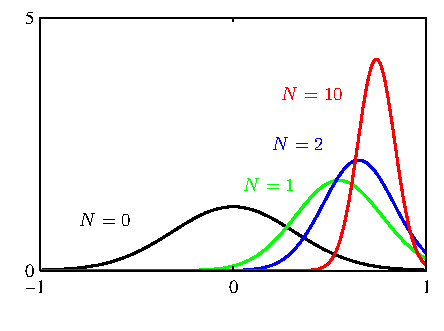
\includegraphics[width=\hsize]{./figs/Figure2_12.pdf}\\Figure 2.12
                \end{figure}
            \end{column}
        \end{columns}
        \begin{itemize}
            \item If we have no observations ($N = 0$), the posterior mean $\mu_N = \mu_0$.
            \item $N \to \infty$ $\Rightarrow$ $\mu_N \to \mu_\mathrm{ML}$ and $\sigma_N^2 \to 0$.
            \item $\sigma_0^2 \to \infty$ (i.e. no prior) $\Rightarrow$ $\mu_N \to \mu_\mathrm{ML}$ and $\sigma_N^2 \to \sigma^2/N$.
        \end{itemize}
    \end{frame}
    
    \begin{frame}{The Bayesian paradigm naturally leads to a sequential view of the inference problem.}
        \begin{align*}
            p(\mu | \mathbf X) &\propto p(\mu)\prod_{n=1}^{N}p(x_n | \mu) \\
            &= \highlightcap<2->[red]{\displaystyle\rbracket{p(\mu)\prod_{n=1}^{N-1}p(x_n | \mu)}}{The posterior after \\ observing $N-1$ data}
            \highlightcap<2->[blue]{p(x_N | \mu)}{The likelihood \\ with $N$-th data} \tag{2.144}
        \end{align*}
        \begin{itemize}
            \item<3-> The posterior after observing $N-1$ data can be viewed as a prior to arriving a posterior after observing $N$-th data.
            \item<3-> The sequential view is very general and applies to any problem in which the observed data are assumed to be i.i.d.
        \end{itemize}
    \end{frame}
    
    \begin{frame}{The task of inferring the precision $\lambda \equiv 1/\sigma^2$ (the mean $\mu$ is known)}
        \begin{itemize}
            \item A set of $N$ observations: $\mathbf X = \cbracket{x_1, \cdots, x_N}$
            \item The likelihood function (the prob. of the observed data given $\lambda$):
                \begin{align*}
                    p(\mathbf X | \lambda) &= \prod_{n=1}^N p(x_n | \lambda) \\
                    &\propto \highlightcap[red]<2->{\lambda^{N/2}}{a power of $\lambda$}\highlightcap<2->[red]{\displaystyle\exp\cbracket{-\frac{\lambda}{2}\sum_{n=1}^N (x_n - \mu)^2}}{the exp of a linear function of $\lambda$} \tag{2.145}
                \end{align*}
            \item The corresponding prior $p(\lambda)$ should be proportional to (2.145).
            \item<3-> We therefore take our prior to be the \textit{gamma distribution}:
                \begin{align*}
                    \mathrm{Gam}(\lambda | a, b) = \frac{1}{\Gamma(a)}b^a\lambda^{a-1}\exp(-b\lambda) \tag{2.146}
                \end{align*}
        \end{itemize}
    \end{frame}

    \begin{frame}{The gamma distribution}
        \begin{align*}
            \mathrm{Gam}(\lambda | a, b) &= \frac{1}{\Gamma(a)}b^a\lambda^{a-1}\exp(-b\lambda) \tag{2.146} \\
            \mathbb E[\lambda] &= \frac{a}{b} \tag{2.147} \\
            \mathrm{var}[\lambda] &= \frac{a}{b^2} \tag{2.148}
        \end{align*}
        \begin{figure}[h]\centering
            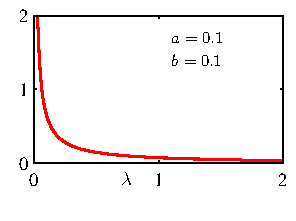
\includegraphics[width=0.3\hsize]{./figs/Figure2_13a.pdf}
            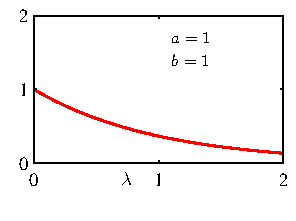
\includegraphics[width=0.3\hsize]{./figs/Figure2_13b.pdf}
            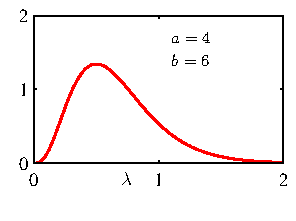
\includegraphics[width=0.3\hsize]{./figs/Figure2_13c.pdf}
        \end{figure}\vspace{-5mm}
        \begin{itemize}
            \item (2.146) is correctly normalized by $\Gamma(a)$ (ex.\ 2.41).
            \item If $a > 0$, the distribution has a finite integral.
            \item If $a \geqslant 1$, the distribution itself is finite.
            \item Derivation of (2.147) and (2.148): ex.\ (2.42)
        \end{itemize}
    \end{frame}

    \begin{supframe}{Solution of Exercise 2.41}
        Easy!
    \end{supframe}
    
    \begin{supframe}{Solution of Exercise 2.42}
        Easy!
    \end{supframe}

    \begin{frame}{The task of inferring the precision $\lambda \equiv 1/\sigma^2$ (the mean $\mu$ is known)}
        \begin{itemize}
            \item The likelihood:
                \begin{align*}
                    p(\mathbf X | \lambda) = \prod_{n=1}^N p(x_n | \lambda) 
                    \propto \lambda^{N/2}\exp\cbracket{-\frac{\lambda}{2}\sum_{n=1}^N (x_n - \mu)^2} \tag{2.145}
                \end{align*}
            \item Consider a prior distribution: $p(\lambda) = \mathrm{Gam}(\lambda | a_0, b_0)$
            \item If we multiply by the likelihood (2.145), then we obtain a posterior:
                \begin{align*}
                    p(\lambda | \mathbf X) 
                    &\propto \lambda^{a_0 - 1}\lambda^{N/2}\exp\cbracket{-b_0\lambda-\frac{\lambda}{2}\sum_{n=1}^N (x_n - \mu)^2} \tag{2.149} \\
                    &= \highlightcap<2->[red]{\lambda^{a_0 + N/2 - 1}}{$\lambda^{a-1}$}
                    \exp\cbracket{\highlightcap<2->[blue]{\displaystyle-\nbracket{b_0+\frac{1}{2}\sum_{n=1}^N (x_n - \mu)^2}\lambda}{$-b\lambda$}}
                \end{align*}
        \end{itemize}
    \end{frame}

    \begin{frame}{The task of inferring the precision $\lambda \equiv 1/\sigma^2$ (the mean $\mu$ is known)}
        \begin{itemize}
            \item Therefore, the posterior is
                \begin{align*}
                    p(\lambda | \mathbf X) &= \mathrm{Gam}(\lambda | a_N, b_N) \\
                    a_N &= a_0 + \frac{N}{2} \tag{2.150} \\
                    b_N &= b_0+\frac{1}{2}\sum_{n=1}^N (x_n - \mu)^2 = b_0 + \frac{N}{2} \sigma_\mathrm{ML}^2\tag{2.151}
                \end{align*}
            \item Interpretation of the posterior's params
                \begin{itemize}
                    \item From (2.150), we see that observing $N$ data increases $a$ by $N/2$.
                \end{itemize}
        \end{itemize}
    \end{frame}

    \begin{frame}{Find a conjugate prior when both the mean and the precision are unknown}
        To find a conjugate prior $p(\mu, \lambda)$, we consider the dependence of the likelihood on $\mu$ and $\lambda$, 
        \begin{align*}
            &p(\mathbf X | \mu, \lambda) = \prod_{n=1}^N \nbracket{\frac{\lambda}{2\pi}}^{1/2}\exp\cbracket{-\frac{\lambda}{2}(x_n - \mu)^2} \\
            &\propto \rbracket{\lambda^{1/2}\exp\nbracket{-\frac{\lambda\mu^2}{2}}}^N
                \exp\cbracket{\lambda\mu \sum_{n=1}^N x_n - \frac{\lambda}{2}\sum_{n=1}^Nx_n^2}\tag{2.152}
        \end{align*}
        The prior $p(\mu, \lambda)$ that has the same functional dependence on $\mu$ and $\lambda$ as the likelihood
        and that should therefore take the form:
        \begin{align*}
            p(\mu, \lambda)
            &\propto \rbracket{\lambda^{1/2}\exp\nbracket{-\frac{\lambda\mu^2}{2}}}^\beta
                \exp\cbracket{c\lambda\mu - d\lambda}\\
            &= \exp\cbracket{-\frac{\beta\lambda}{2}(\mu - c/\beta)^2}\lambda^{\beta/2}\exp\cbracket{-\nbracket{d - \frac{c^2}{2\beta}}\lambda}
                \tag{2.153}
        \end{align*}
    \end{frame}

    \begin{frame}{Find a conjugate prior when both the mean and the precision are unknown}
        \begin{itemize}
            \item Recall we can always write $p(\mu, \lambda) = \highlight<2->[red]{p(\mu | \lambda)}\highlight<2->[blue]{p(\lambda)}$.
                \begin{align*}
                    p(\mu, \lambda)
                    \propto
                        \highlightcap<2->[red]{\displaystyle\exp\cbracket{-\frac{\beta\lambda}{2}(\mu - c/\beta)^2}}{Gaussian}
                        \highlightcap<2->[blue]{\displaystyle\lambda^{\beta/2}\exp\cbracket{-\nbracket{d - \frac{c^2}{2\beta}}\lambda}}{gamma distribution} \tag{2.153}
                \end{align*}
            \item<3-> By defining new constants $\mu_0 = c/\beta$, $a = (1 + \beta) / 2$ and $b = d - c^2/2\beta$, and normalizing (2.153),
                we obtain the \textit{normal-gamma} distribution:
                \begin{align*}
                    p(\mu, \lambda) = \mathcal N(\mu | \mu_0, (\beta\lambda)^{-1}) \mathrm{Gam}(\lambda | a, b) \tag{2.154}
                \end{align*}
            \item<3-> NOTE: This dist is not simply the product of an independent Gaussian prior and a gamma prior.
        \end{itemize}
    \end{frame}

    \begin{frame}{Summary: conjugate priors in the case of the univariate Gaussian}

    \end{frame}

    \begin{frame}{In the case of the multivariate Gaussian $\mathcal N(\mathbf x | \bm\mu, \bm\Lambda^{-1})$ for a $D$-dim vector $\mathbf x$}
        \begin{itemize}
            \item For known mean $\bm\mu$ and unknown precision $\bm\Lambda$, the conjugate prior is a Gaussian:
                $p(\bm\mu) = \mathcal N(\bm\mu | \bm\mu_0, \bm\Lambda_0^{-1})$
            \item For unknown mean $\bm\mu$ and known precision $\bm\Lambda$, the conjugate prior is the \textit{Wishart} distribution:
                \begin{align*}
                    p(\bm\Lambda) = \mathcal W(\bm\Lambda | \mathbf W, \nu)
                    = B |\bm\Lambda|^{(\nu - D - 1)/2}\exp\nbracket{-\frac{1}{2}\tr(\mathbf W^{-1}\bm\Lambda)} \tag{2.155}
                \end{align*}
                \vspace{-7.5mm}
                \begin{itemize}
                    \item $\nu$ is the number of \textit{degrees of freedom}.
                    \item $\mathbf W \in \mathbb R^{D\times D}$
                    \item $B$ is a nomalization constant (2.156).
                \end{itemize}
            \item For both the mean and the precision are unknown, the conjugate prior is the \textit{normal-Wishart} distribution:
                \begin{align*}
                    p(\bm\mu, \bm\Lambda | \bm\mu_0, \beta, \mathbf W, \nu)
                    = \mathcal N(\bm\mu | \bm\mu_0, (\beta\bm\Lambda)^{-1}) \mathcal W(\bm\Lambda | \mathbf W, \nu) \tag{2.157}
                \end{align*}
        \end{itemize}
    \end{frame}

    \begin{frame}{A conjugate prior over the variance and the covariance}
        \begin{itemize}
            \item Instead of working with the precision, we can consider the variance (covariance) itself.
                The conjugate priors are called:
                \begin{itemize}
                    \item the \textit{inverse gamma} distribution (the univariate Gaussian case)
                    \item the \textit{inverse Wishart} distribution (the multivariate Gaussian case)
                \end{itemize}
            \item We shall not discuss this further because we will find it more convenient to work with the precision.
        \end{itemize}
    \end{frame}

    \section{\S2.3.7 Student's t-distribution}

    \begin{frame}{Marginalize the precision using a gamma prior}
        \begin{itemize}
            \item We have seen that the conj prior for the precision of Gaussian is given by a gamma dist.
            \item If we have $\mathcal N(x | \mu, \tau^{-1})$ together with a Gamma prior $\mathrm{Gam}(\tau | a, b)$
                and integrate out the precision, we obtain the marginal dist of $x$:\\
                (derivation: ex.\ 2.46)
                \begin{align*}
                    p(x | \mu, a, b) &= \int p(x, \tau | \mu, a, b) \:\mathrm d\tau \\
                    &= \int_0^\infty \mathcal N(x | \mu, \tau^{-1}) \mathrm{Gam}(\tau | a, b) \:\mathrm d\tau \tag{2.158} \\
                    &= \frac{b^a}{\Gamma(a)}\nbracket{\frac{1}{2\pi}}^{1/2}\rbracket{b + \frac{(x - \mu)^2}{2}}^{-a-1/2}\Gamma(a+1/2)
                \end{align*}
            \item By convention we define $\nu = 2a$ and $\lambda = a / b$, and obtain the \textit{Student's t-distribution}:
                \begin{align*}
                    \mathrm{St}(x | \mu, \lambda, \nu)
                    = \frac{\Gamma(\nu/2+1/2)}{\Gamma(\nu / 2)} \nbracket{\frac{\lambda}{\pi\nu}}^{1/2}
                        \rbracket{1 + \frac{\lambda(x-\mu)^2}{\nu}}^{-\nu/2-1/2} \tag{2.159}
                \end{align*}
        \end{itemize}
    \end{frame}
    
    \begin{supframe}{Solution of Exercise 2.46}
        Use $\displaystyle \Gamma(a) = \int_0^\infty t^{a-1}e^{-t} \:\mathrm dt = \int_0^\infty (Au)^{a-1}e^{-Au} A \:\mathrm du$.
        \begin{align*}
            &p(x | \mu, a, b) = \int_0^\infty \mathcal N(x | \mu, \tau^{-1}) \mathrm{Gam}(\tau | a, b) \:\mathrm d\tau \tag{2.158} \\
            &= \int_0^\infty \nbracket{\frac{\tau}{2\pi}}^{\frac{1}{2}}
                \exp\nbracket{-\frac{\tau}{2}(x - \mu)^2}\cdot\frac{1}{\Gamma(a)}b^a\tau^{a-1}\exp(-b\tau)\:\mathrm d\tau \\
            &= \frac{b^a}{\Gamma(a)}\nbracket{\frac{1}{2\pi}}^{1/2}
                \int_0^\infty \tau^{(a+1/2)-1} \exp\cbracket{-\highlightcap[red]{\displaystyle \nbracket{b + \frac{(x-\mu)^2}{2}}}{$\equiv A$}\tau} \:\mathrm d\tau \\
            &= \frac{b^a}{\Gamma(a)}\nbracket{\frac{1}{2\pi}}^{1/2}\frac{1}{A^{(a+1/2)-1}A}
                \highlightcap[blue]{\displaystyle\int_0^\infty (A\tau)^{(a+1/2)-1} \exp\cbracket{-\highlight[red]{A}\tau}  A \:\mathrm d\tau}{$\Gamma(a+1/2)$} \\
            &= \frac{b^a}{\Gamma(a)}\nbracket{\frac{1}{2\pi}}^{1/2}\rbracket{b + \frac{(x - \mu)^2}{2}}^{-a-1/2}\Gamma(a+1/2)
        \end{align*}
    \end{supframe}

    \begin{frame}{Student's t-distribution}
        \begin{align*}
            \mathrm{St}(x | \mu, \lambda, \nu)
            = \frac{\Gamma(\nu/2+1/2)}{\Gamma(\nu / 2)} \nbracket{\frac{\lambda}{\pi\nu}}^{1/2}
                \rbracket{1 + \frac{\lambda(x-\mu)^2}{\nu}}^{-\nu/2-1/2} \tag{2.159}
        \end{align*}\vspace{-4mm}
        \begin{itemize}
            \item $\lambda$: the \textit{precision} of t-distribution \\ (NOTE: it is not  in general equal to the inverse of the variance)
            \item $\nu$: the \textit{degrees of freedom}
            \item When $\nu = 1$, it reduces to the \textit{Cauchy} dist.
            \item When $\nu \to \infty$, it becomes a Gaussian $\mathcal N(x | \mu, \lambda^{-1})$ (ex.\ 2.47).
        \end{itemize}
        \begin{figure}[h]\centering
            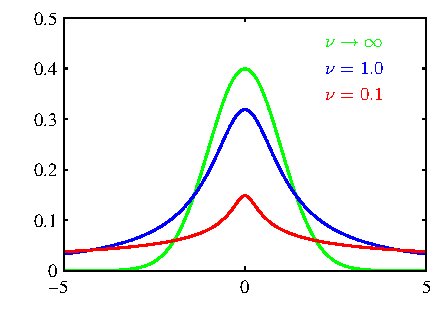
\includegraphics[height=3.5cm]{./figs/Figure2_15.pdf}
        \end{figure}
    \end{frame}

    \begin{supframe}{Exercise 2.47}
        Hello metropolis!
    \end{supframe}

    \begin{frame}{Properties of the t-distribution (1/2): the robustness}
        Hello metropolis!
    \end{frame}

    \begin{frame}{Title}
        Hello metropolis!
    \end{frame}

    \begin{frame}{Title}
        Hello metropolis!
    \end{frame}

\end{document}
